%!TEX TS-program = xelatex
%!TEX encoding = UTF-8 Unicode
%!TEX root = 2020-GS-ARTICLE.tex
%----------------------------------------------------------------- LANGUAGES ---
\newcommand{\mylanguages}{italian,english} % in reverse order
%---------------------------------------------------------- TITLE & SUBTITLE ---
\newcommand{\mytitle}{Ambiophonic Reverberation}
\newcommand{\mysubtitle}{For a more accessible and less technical introduction
                         to this topic, \\ see Introduction to General Relativity}
%----------------------------------------------------------------- AUTHOR(s) ---
\newcommand{\authorone}{Paradisi Francesco}
\newcommand{\institutione}{Conservatorio S. Cecilia di Roma}
\newcommand{\emailone}{francesco.paradisi10@ gmail.com}
%-------------------------------------------------------------------------------
\newcommand{\authortwo}{Giuseppe Silvi}
\newcommand{\institutiontwo}{Conservatorio Nicolini di Bari}
\newcommand{\emailtwo}{silvi.giuseppe @ docenticonsba.it} % duplicate these 3 lines if more
%-------------------------------------------------------------------------------
\newcommand{\authorthree}{Edoardo Staffa}
\newcommand{\institutionthree}{Conservatorio S. Cecilia di Roma}
\newcommand{\emailthree}{edoardo.staffa1 @ gmail.com} % duplicate these 3 lines if more
%-------------------------------------------------------------- STYLE GS2020 ---
%!TEX TS-program = xelatex
%!TEX encoding = UTF-8 Unicode
%!TEX root = 2020-GS-ARTICLE.tex
%-------------------------------- PACKAGES AND OTHER DOCUMENT CONFIGURATIONS ---
\documentclass[
	a4paper,
	twocolumn
]{article}
\usepackage[
	top=20mm,
	bottom=25mm,
	textwidth=17.2cm,
	columnsep=0.8cm
]{geometry}
\usepackage[T1]{fontenc}
\usepackage[\mylanguages]{babel}
\usepackage{graphicx}
\usepackage{dblfloatfix}
\usepackage{graphicx}
\usepackage{epstopdf}
\epstopdfsetup{update}
\usepackage[usenames]{color}
\usepackage{xcolor}
\usepackage{amssymb}
\usepackage{hyperref} % For hyperlinks in the PDF
\usepackage{Alegreya}
\linespread{1.05}
\usepackage{
	fontspec,
	xltxtra,
	xunicode
	}
\usepackage{
	xfrac,
	unicode-math
	}

\defaultfontfeatures{Mapping=tex-text}
\setmonofont[
	Scale=MatchLowercase
	]{Andale Mono}
\setmathfont[
	Scale=MatchLowercase,
	Scale=1
	]{Libertinus Math}

\usepackage{microtype}

\usepackage[
	hang,
	small,
	labelfont=bf,
	up,
	textfont=it,
	up
	]{caption}
\usepackage{paralist} % For compact item lists
\usepackage{etoolbox} % Some tools: used for quote environment
\AtBeginEnvironment{quote}{\small}
\usepackage{titling} % Customizing the title section
\usepackage{booktabs} % Horizontal rules in tables
\usepackage{enumitem} % Customized lists
\setlist[itemize]{noitemsep} % Make itemize lists more compact
\usepackage{abstract} % Allows abstract customization
\renewcommand{\abstractnamefont}{\normalfont\bfseries} % Set the "Abstract" text to bold
\renewcommand{\abstracttextfont}{\normalfont\small\itshape} % Set the abstract itself to small italic text
\usepackage{titlesec} % Allows customization of titles
\renewcommand\thesection{\Roman{section}} % Roman numerals for the sections
\renewcommand\thesubsection{\Roman{subsection}} % roman numerals for subsections
\titleformat{\section}[block]{\large\centering}{\thesection.}{1em}{} % Change the look of the section titles
\titleformat{\subsection}[block]{\large}{\thesubsection.}{1em}{} % Change the look of the section titles
%------------------------------------------------------------- TITLE SECTION ---
\setlength{\droptitle}{-4\baselineskip} % Move the title up
\pretitle{\begin{center}\huge\bfseries} % Article title formatting
\posttitle{\end{center}} % Article title closing formatting
\title{\mytitle \\ \large{\emph{\mysubtitle}}} % Article title
\author{%
\textsc{\authorone}\\%
\normalsize \institutione \\ %
\normalsize \emailone%
\and
\textsc{\authortwo} \\%
\normalsize \institutiontwo \\ %
\normalsize \emailtwo %
\and
\textsc{\authorthree} \\%
\normalsize \institutionthree \\ %
\normalsize \emailthree %
}
\date{} % Leave empty to omit a date

\usepackage{fancyhdr} % Headers and footers
\pagestyle{fancy} % All pages have headers and footers
\fancyhead{} % Blank out the default header
\fancyfoot{} % Blank out the default footer
\fancyhead[C]{\small Ambiophonic Reverberation • Research Notes} % Custom header text
\fancyfoot[RO,LE]{\small \today~ • w: \input{includes/words.txt} • c: \input{includes/char.txt} • p:~\thepage} % Custom footer text
%-------------------------------------------------------------------------------
%-------------------------------------------------------------------------------
%	LISTINGS
%-------------------------------------------------------------------------------
%-------------------------------------------------------------------------------
\usepackage{listings}
% lstlistings setup
\definecolor{gsbg}{rgb}{0.98,0.98,0.98}

\lstset{%
  aboveskip=10pt,
	belowskip=5pt,
  language=C++,
  numbers=none,%left,%none,
  tabsize=4,
  %frame=single,
  breaklines=true,
  numberstyle=\tiny\ttfamily,
  backgroundcolor=\color{gsbg},
  basicstyle=\footnotesize\ttfamily,
  %commentstyle=\slshape\color{mylstcmt}, %\itshape,
  %frameround=tttt,
  columns=flexible, %fixed,
  showstringspaces=false,
  emptylines=2,
  inputencoding=utf8,
  extendedchars=true,
  literate=	{á}{{\'a}}1
			{à}{{\`a}}1
			{ä}{{\"a}}1
			{â}{{\^a}}1
			{é}{{\'e}}1
			{è}{{\`e}}1
			{ë}{{\"e}}1
			{ê}{{\^e}}1
			{ï}{{\"i}}1
			{î}{{\^i}}1
			{ö}{{\"o}}1
			{ô}{{\^o}}1
			{è}{{\`e}}1
			{ù}{{\`u}}1
			{û}{{\^u}}1
			{ç}{{\c{c}}}1
			{Ç}{{\c{C}}}1,
  emph={component, declare, environment, import, library, process},
  emph={[2]ffunction, fconstant, fvariable},
  emph={[3]button, checkbox, vslider, hslider, nentry, vgroup, hgroup, tgroup, vbargraph, hbargraph, attach},
  %emphstyle=\color{yotxt}, %\underline, %\bfseries,
  %morecomment=[s][\color{mylstdoc}]{<mdoc>}{</mdoc>},
  rulecolor=\color{black}
}

\usepackage[framemethod=tikz]{mdframed} % Allows defining custom boxed/framed environments

%-------------------------------------------------------------------------------
%--------------------------------------------------- INFORMATION ENVIRONMENT ---
%-------------------------------------------------------------------------------

% Usage:
% \begin{info}[optional title, defaults to "Info:"]
% 	contents
% 	\end{info}

\mdfdefinestyle{info}{%
	topline=false, bottomline=false,
	leftline=false, rightline=false,
	nobreak,
	singleextra={%
		\fill[black](P-|O)circle[radius=0.4em];
		\node at(P-|O){\color{white}\scriptsize\bf i};
		\draw[very thick](P-|O)++(0,-0.8em)--(O);%--(O-|P);
	}
}

% Define a custom environment for information
\newenvironment{info}[1][Info:]{ % Set the default title to "Info:"
	\medskip
	\begin{mdframed}[style=info]
		\noindent{\textbf{#1}}
}{
	\end{mdframed}
}

%-------------------------------------------------------------------------------
%----------------------------------------------------- BIOGRAFIA ENVIRONMENT ---
%-------------------------------------------------------------------------------

% Usage:
% \begin{bio}[optional title, defaults to "Info:"]
% 	contents
% 	\end{bio}

\mdfdefinestyle{bio}{%
	topline=false, bottomline=false,
	leftline=false, rightline=false,
	nobreak,
	singleextra={%
		\fill[black](P-|O)circle[radius=0.4em];
		\node at(P-|O){\color{white}\scriptsize\bf b};
		\draw[very thick](P-|O)++(0,-0.8em)--(O);%--(O-|P);
	}
}

% Define a custom environment for information
\newenvironment{bio}[1][Biografia:]{ % Set the default title to "Info:"
	\medskip
	\begin{mdframed}[style=bio]
		\noindent{\textbf{#1}}
}{
	\end{mdframed}
}

%-------------------------------------------------------------------------------
%------------------------------------------------------- WARNING ENVIRONMENT ---
%-------------------------------------------------------------------------------

% Usage:
% \begin{warn}[optional title, defaults to "Warning:"]
%	Contents
% \end{warn}

\mdfdefinestyle{warning}{
	topline=false, bottomline=false,
	leftline=false, rightline=false,
	nobreak,
	singleextra={%
		\draw(P-|O)++(-0.5em,0)node(tmp1){};
		\draw(P-|O)++(0.5em,0)node(tmp2){};
		\fill[black,rotate around={45:(P-|O)}](tmp1)rectangle(tmp2);
		\node at(P-|O){\color{white}\scriptsize\bf !};
		\draw[very thick](P-|O)++(0,-1em)--(O);%--(O-|P);
	}
}

% Define a custom environment for warning text
\newenvironment{warn}[1][Warning:]{ % Set the default warning to "Warning:"
	\medskip
	\begin{mdframed}[style=warning]
		\noindent{\textbf{#1}}
}{
	\end{mdframed}
}

%-------------------------------------------------------------------- ABSTRACT -
\renewcommand{\maketitlehookd}{%
\begin{abstract}
\noindent\input{includes/abstract.txt}
\end{abstract}
}

%------------------------------------------------------------ BEGIN DOCUMENT ---
\begin{document}
\maketitle
\thispagestyle{empty}
%-------------------------------------------------------------------- ABSTRACT -
% The abstract is an external txt file inside the includes folder
%-------------------------------------------------------------------------------
\section*{TO DO LIST}
\begin{compactitem}
\item analisi della bibliografia
\item descrizione generica dell'algoritmo di schroeder
\item le potenzialità dell'algoritmo
\item implementazione algoritmo in faust
\item allestimento dell'ambiophonic reverberation in sala concerto
\item implementazione esplicativa per Live Electronics
\item conclusioni
\item
\item
\end{compactitem}
%-------------------------------------------------------------------------------
\subsection*{UNNUMBERED SUB-SECTION}

\begin{warn}[Einstein's theory]
 has important astrophysical implications. For example, it
implies the existence of black holes regions of space in which space and time
are distorted in such a way that nothing, not even light, can escape as an
end state for massive stars.
\end{warn}

There is ample evidence that the intense radiation
emitted by certain kinds of astronomical objects is due to black holes. For
example, microquasars and active galactic nuclei result from the presence of
stellar black holes and supermassive black holes, respectively. The bending of
light by gravity can lead to the phenomenon of gravitational lensing, in which
multiple images of the same distant astronomical object are visible in the sky.
General relativity also predicts the existence of gravitational waves, which
have since been observed directly by the physics collaboration LIGO.
%-------------------------------------------------------------------------------
\subsubsection*{UNNUMBERED SUB-SUB-SECTION}
Some predictions of general relativity differ significantly from those of
classical physics, especially concerning the passage of time, the geometry of
space, the motion of bodies in free fall, and the propagation of light. Examples
of such differences include gravitational time dilation, gravitational lensing,
the gravitational redshift of light, and the gravitational time delay. The
predictions of general relativity in relation to classical physics have been
confirmed in all observations and experiments to date. Although general
relativity is not the only relativistic theory of gravity, it is the simplest
theory that is consistent with experimental data. However, unanswered questions
remain, the most fundamental being how general relativity can be reconciled with
the laws of quantum physics to produce a complete and self-consistent theory of
quantum gravity.

Einstein's theory has important astrophysical implications. For example, it
implies the existence of black holes regions of space in which space and time
are distorted in such a way that nothing, not even light, can escape as an
end state for massive stars. There is ample evidence that the intense radiation
emitted by certain kinds of astronomical objects is due to black holes. For
example, microquasars and active galactic nuclei result from the presence of
stellar black holes and supermassive black holes\ldots


\vfill\null

\begin{figure}[b]
\begin{center}
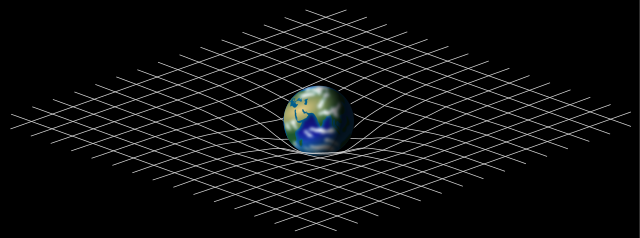
\includegraphics[width=.47\textwidth]{img/image1.png}
\caption{\textbf{Spacetime curvature schematic}. Lattice analogy of the deformation
of spacetime caused by a planetary mass.}
\label{gr01}
\end{center}
\end{figure}

\newpage % USE NEWPAGE TO FORCE COLUMNN INTERRUPTION
%-------------------------------------------------------------------------------
%-------------------------------------------------------------------------------
\section*{UNNUMBERED SECTION}

\begin{quote}
La musica non e` solo composizione. \\
Non è artigianato, non è un mestiere. \\
La musica è pensiero. \cite{nono85}
\end{quote}

Some predictions of general relativity differ significantly from those of
classical physics, especially concerning the passage of time, the geometry of
space, the motion of bodies in free fall, and the propagation of light. Examples
of such differences include gravitational time dilation, gravitational lensing,
the gravitational redshift of light, and the gravitational time delay. The
predictions of general relativity in relation to classical physics have been
confirmed in all observations and experiments to date. Although general
relativity is not the only relativistic theory of gravity, it is the simplest
theory that is consistent with experimental data. However, unanswered questions
remain, the most fundamental being how general relativity can be reconciled with
the laws of quantum physics to produce a complete and self-consistent theory of
quantum gravity.

\begin{table}[htp]
\begin{center}
\begin{tabular}{ll}
\textbf{Stages} & \textbf{Dur.} \\
\hline
\textbf{Omnidirectional Expositions} & 6 mo. \\
Sound-shape analysis and visualizations & \\
Sound-shape reproduction & \\
Sound-shape database design & \\
\hline
\textbf{Micro-Rhythm of sound-shape} & 12 mo. \\
Solo repertoire analysis & \\
Sound-shape explosion in practising & \\
From literature to shapes open-data & \\
\hline
\textbf{Rhythm of sound-shape interactions} & 12 mo. \\
Multiple sources multiple shapes & \\
Relationship and complexity perception & \\
\hline
\textbf{Sound-shape in musical composition} & 12 mo. \\
AI: unleashed writing opportunities & \\
AI: can you listen the time? & \\
\hline
\textbf{Final documentation} & 6 mo. \\
\end{tabular}
\label{timesheet}
\caption{Thinking Tetrahedral Today stages}
\end{center}
\end{table}%

Einstein's theory has important astrophysical implications. For example, it
implies the existence of black holes regions of space in which space and time
are distorted in such a way that nothing, not even light, can escape as an
end state for massive stars. There is ample evidence that the intense radiation
emitted by certain kinds of astronomical objects is due to black holes. For
example, microquasars and active galactic nuclei result from the presence of
stellar black holes and supermassive black holes, respectively. The bending of
light by gravity can lead to the phenomenon of gravitational lensing, in which
multiple images of the same distant astronomical object are visible in the sky.
General relativity also predicts the existence of gravitational waves, which
have since been observed directly by the physics collaboration LIGO. In addition,
general relativity is the basis of current cosmological models of a consistently
expanding universe. \cite{gerzon_70b}

\begin{compactitem}
\item Derivations of the Lorentz transformations
\item Einstein–Hilbert action
\item Tests of general relativity
\item Two-body problem in general relativity
\end{compactitem}

\begin{figure}[t]
\centering

\includegraphics[width=.47\textwidth]{img/image2.jpg}
\caption{Mind Mapping}
\label{gs}
\end{figure}

\begin{equation}
m(x,p,\theta) = (p*x) + ((1-p)*(x\cos\theta)
\label{eq:mid}
\end{equation}

Some predictions of general relativity differ significantly from those of
classical physics, especially concerning the passage of time, the geometry of
space, the motion of bodies in free fall, and the propagation of light.

%--------------------------------------------
%----------------larghezza massima del codice
\begin{lstlisting}
mspan(x,p,rad) = m,s
with{
  m = (p*x)+((1-p)*(x*cos(rad)));
  s = x*(sin(-rad));
};
\end{lstlisting}

Examples of such differences include gravitational time dilation, gravitational
lensing, the gravitational redshift of light, and the gravitational time delay.
The predictions of general relativity in relation to classical physics have been
confirmed in all observations and experiments to date.

\vfill\null

\raggedright
\bibliographystyle{unsrt}
\bibliography{includes/bibliography.bib}

\end{document}

%%%%%%%%%%%%%%%%%%%%%%%%%%%%%%%%%%%%%%%%%%%%%%%%%%%%%%%%%%%%%%%%%%%%%%%%%%%%%%%%
% 2020 GIUSEPPE SILVI ARTICLE TEMPLATE BASED ON
%%%%%%%%%%%%%%%%%%%%%%%%%%%%%%%%%%%%%%%%%%%%%%%%%%%%%%%%%%%%%%%%%%%%%%%%%%%%%%%%
% Journal Article
% LaTeX Template
% Version 1.4 (15/5/16)
% This template has been downloaded from:
% http://www.LaTeXTemplates.com
% Original author:
% Frits Wenneker (http://www.howtotex.com) with extensive modifications by
% Vel (vel@LaTeXTemplates.com)
% License:
% CC BY-NC-SA 3.0 (http://creativecommons.org/licenses/by-nc-sa/3.0/)
%%%%%%%%%%%%%%%%%%%%%%%%%%%%%%%%%%%%%%%%%%%%%%%%%%%%%%%%%%%%%%%%%%%%%%%%%%%%%%%%
